
\medskip

Un entraîneur de sport prépare deux circuits d'entraînement contenant plusieurs exercices de cardio et de renforcement musculaire :

\begin{itemize}[label=\textbullet]
	\item un circuit commence à l'exercice 1 et se termine en revenant à l'exercice 1;
	\item le circuit 1 contient cinq exercices. Chaque exercice dure 40 secondes et doit être suivi de 16 secondes de repos permettant de se rendre à l'exercice suivant;
	\item le circuit 2 contient dix exercices. Chaque exercice dure 30 secondes et doit être suivi de 5 secondes de repos permettant de se rendre à l'exercice suivant.
\end{itemize}

\begin{center}
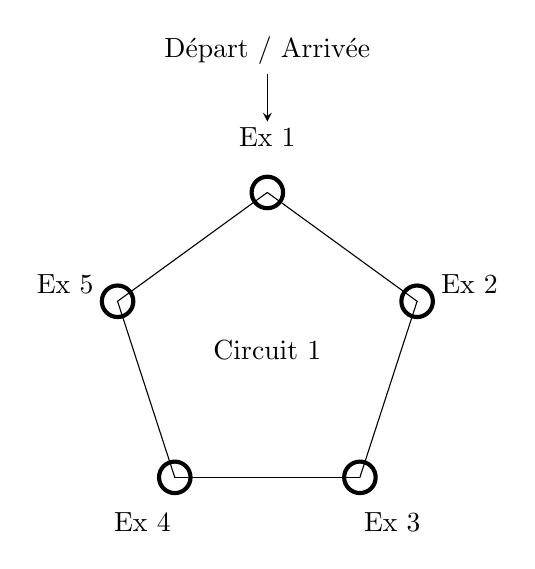
\begin{tikzpicture}[line cap=round,baseline={(C)}]
		\draw[<-, >=stealth] (0,2.9)--(0,3.5) node[above]{Départ / Arrivée};
		\foreach \ex in {1,...,5}{
			\draw[line width=1.5pt] (162-\ex*72:2)circle (0.2);
			\node at (162-\ex*72:2.7) {Ex~\ex};
			\draw (162-\ex*72:2)--(90-\ex*72:2);}
		\node (C) at(0,0) {Circuit 1};
\end{tikzpicture}
\hfill~
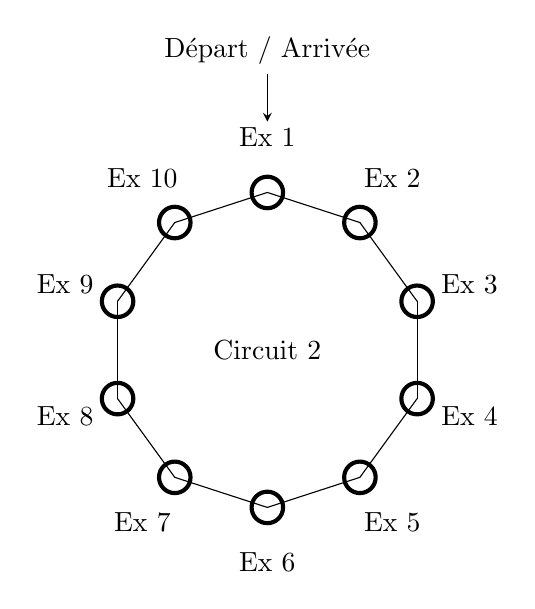
\begin{tikzpicture}[line cap=round,baseline={(C)}]
		\draw[<-, >=stealth] (0,2.9)--(0,3.5) node[above]{Départ / Arrivée};
		\foreach \ex in {1,...,10}{
			\draw[line width=1.5pt] (126-\ex*36:2)circle (0.2);
			\node at (126-\ex*36:2.7) {Ex~\ex};
			\draw (126-\ex*36:2)--(90-\ex*36:2);}
		\node (C) at(0,0) {Circuit 2};
\end{tikzpicture}

\end{center}

\begin{enumerate}
\item Montrer que le circuit 1 s'effectue en 280 secondes et que le circuit 2 s'effectue en 350 secondes.
\item Donner la décomposition en produit de facteurs premiers de $280$ et de $350$.
\item Une séance d'entraînement est constituée de plusieurs tours du même circuit.

Au coup de sifflet de l'entraîneur, Camille commence une séance d'entraînement sur le circuit 1 et Dominique sur le circuit 2.

	\begin{enumerate}
		\item Expliquer pourquoi, lorsque \np{2800} secondes se sont écoulées à partir du coup de sifflet, Camille se trouve de nouveau au départ du circuit 1.

		Préciser où se trouve Dominique sur le circuit 2 lorsque \np{2800} secondes se sont écoulées.

		\item Après le coup de sifflet, combien de temps faut-il à Camille et Dominique pour se retrouver en même temps pour la première fois au départ de leur circuit ? Exprimer cette durée en minute et seconde.
	\end{enumerate}
\end{enumerate}


